\documentclass{standalone}
\usepackage{tikz}
\usetikzlibrary{patterns, positioning}
\usepackage[sfdefault]{ClearSans} %% option 'sfdefault' activates Clear Sans as the default text font
\usepackage[T1]{fontenc}

\begin{document}
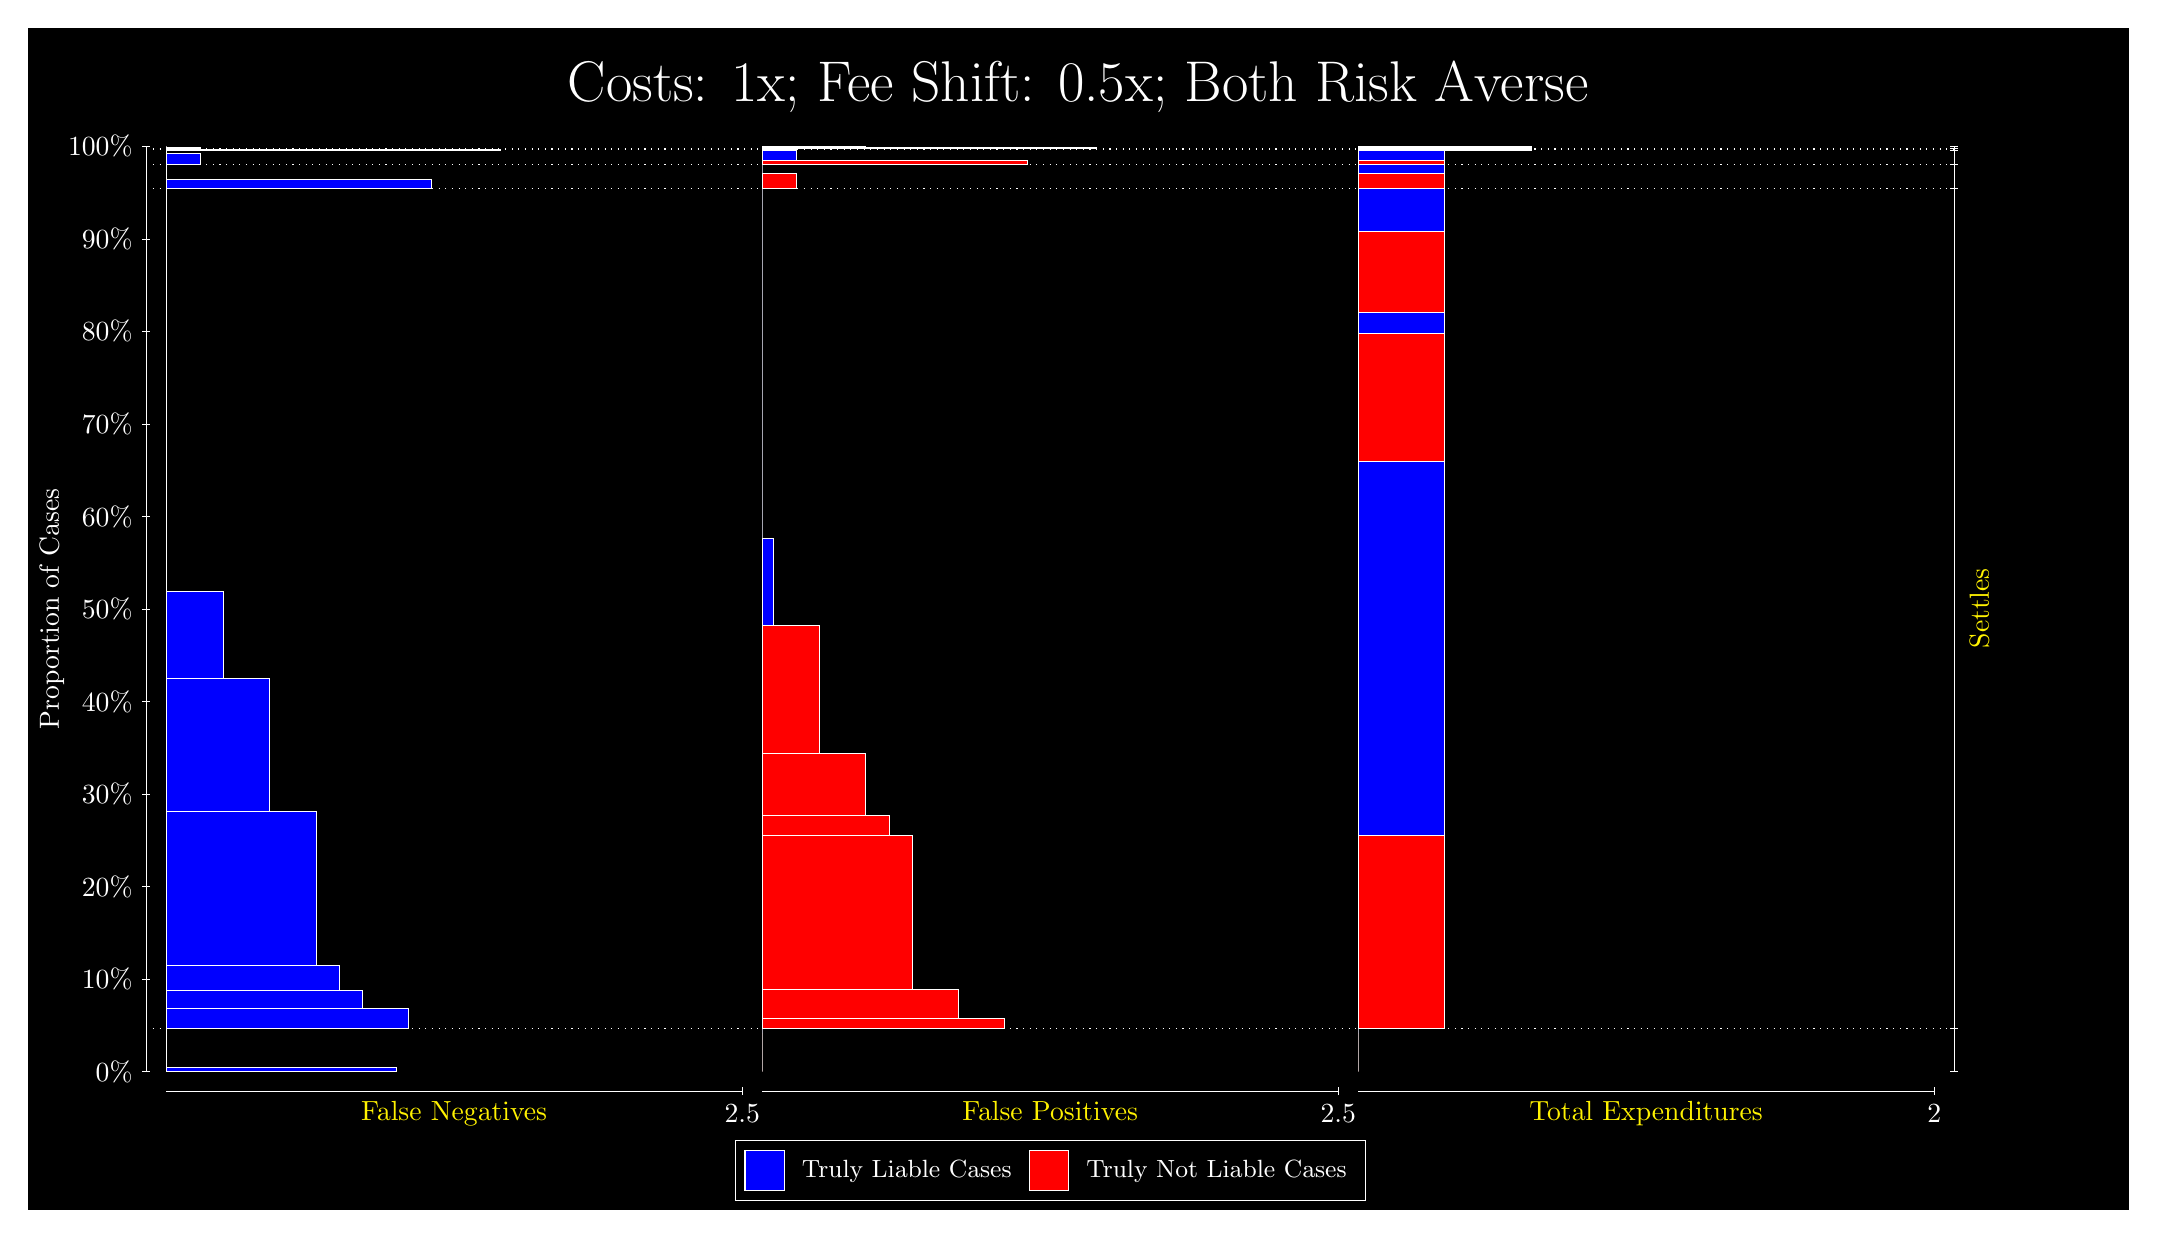
\begin{tikzpicture}
\draw[fill=black] (0,0) rectangle (26.667,15);
\draw[text=white] (0,13.5) rectangle (26.667,15) node[midway] {\huge Costs: 1x; Fee Shift: 0.5x; Both Risk Averse};
\draw[white, very thin] (1.5,1.75) -- (1.5,13.5);
\node[rotate=90, text=white, anchor=center] at (0.3, 7.625) {Proportion of Cases};
\draw[white, very thin] (1.45,1.75) -- (1.55,1.75);
\node[text=white, anchor=east] at (1.45, 1.75) {0\%};
\draw[white, very thin] (1.45,2.925) -- (1.55,2.925);
\node[text=white, anchor=east] at (1.45, 2.925) {10\%};
\draw[white, very thin] (1.45,4.1) -- (1.55,4.1);
\node[text=white, anchor=east] at (1.45, 4.1) {20\%};
\draw[white, very thin] (1.45,5.275) -- (1.55,5.275);
\node[text=white, anchor=east] at (1.45, 5.275) {30\%};
\draw[white, very thin] (1.45,6.45) -- (1.55,6.45);
\node[text=white, anchor=east] at (1.45, 6.45) {40\%};
\draw[white, very thin] (1.45,7.625) -- (1.55,7.625);
\node[text=white, anchor=east] at (1.45, 7.625) {50\%};
\draw[white, very thin] (1.45,8.8) -- (1.55,8.8);
\node[text=white, anchor=east] at (1.45, 8.8) {60\%};
\draw[white, very thin] (1.45,9.975) -- (1.55,9.975);
\node[text=white, anchor=east] at (1.45, 9.975) {70\%};
\draw[white, very thin] (1.45,11.15) -- (1.55,11.15);
\node[text=white, anchor=east] at (1.45, 11.15) {80\%};
\draw[white, very thin] (1.45,12.325) -- (1.55,12.325);
\node[text=white, anchor=east] at (1.45, 12.325) {90\%};
\draw[white, very thin] (1.45,13.5) -- (1.55,13.5);
\node[text=white, anchor=east] at (1.45, 13.5) {100\%};

\draw[white, very thin] (24.457,1.75) -- (24.457,13.5);
\draw[white, very thin] (24.407,1.75) -- (24.507,1.75);
\node[anchor=west] at (24.407, 1.75) {};
\draw[white, very thin] (24.407,2.2966) -- (24.507,2.2966);
\node[anchor=west] at (24.407, 2.2966) {};
\draw[white, very thin] (24.407,12.97) -- (24.507,12.97);
\node[anchor=west] at (24.407, 12.97) {};
\draw[white, very thin] (24.407,13.273) -- (24.507,13.273);
\node[anchor=west] at (24.407, 13.273) {};
\draw[white, very thin] (24.407,13.456) -- (24.507,13.456);
\node[anchor=west] at (24.407, 13.456) {};
\draw[white, very thin] (24.407,13.475) -- (24.507,13.475);
\node[anchor=west] at (24.407, 13.475) {};
\draw[white, very thin] (24.407,13.5) -- (24.507,13.5);
\node[anchor=west] at (24.407, 13.5) {};

\draw[white, very thin, fill=blue] (1.75,1.75) rectangle (4.6775,1.8075);
\draw[white, very thin, fill=red] (1.75,1.8075) rectangle (1.75,2.2966);
\draw[white, very thin, fill=blue] (1.75,2.2966) rectangle (4.8239,2.5516);
\draw[white, very thin, fill=blue] (1.75,2.5516) rectangle (4.2384,2.7768);
\draw[white, very thin, fill=blue] (1.75,2.7768) rectangle (3.9457,3.0945);
\draw[white, very thin, fill=blue] (1.75,3.0945) rectangle (3.6529,5.0559);
\draw[white, very thin, fill=blue] (1.75,5.0559) rectangle (3.0674,6.7431);
\draw[white, very thin, fill=blue] (1.75,6.7431) rectangle (2.4819,7.8436);
\draw[white, very thin, fill=red] (1.75,7.8436) rectangle (1.75,12.97);
\draw[white, very thin, fill=blue] (1.75,12.97) rectangle (5.1167,13.083);
\draw[white, very thin, fill=red] (1.75,13.083) rectangle (1.75,13.273);
\draw[white, very thin, fill=blue] (1.75,13.273) rectangle (2.1891,13.406);
\draw[white, very thin, fill=red] (1.75,13.406) rectangle (1.75,13.456);
\draw[white, very thin, fill=blue] (1.75,13.456) rectangle (5.9949,13.463);
\draw[white, very thin, fill=red] (1.75,13.463) rectangle (1.75,13.475);
\draw[white, very thin, fill=blue] (1.75,13.475) rectangle (2.1891,13.493);
\draw[white, very thin, fill=red] (1.75,13.493) rectangle (1.75,13.5);
\draw[white, very thin, fill=red] (9.3189,1.75) rectangle (9.3189,2.2391);
\draw[white, very thin, fill=blue] (9.3189,2.2391) rectangle (9.3189,2.2966);
\draw[white, very thin, fill=red] (9.3189,2.2966) rectangle (12.393,2.427);
\draw[white, very thin, fill=red] (9.3189,2.427) rectangle (11.807,2.7926);
\draw[white, very thin, fill=red] (9.3189,2.7926) rectangle (11.222,4.7542);
\draw[white, very thin, fill=red] (9.3189,4.7542) rectangle (10.929,5.0046);
\draw[white, very thin, fill=red] (9.3189,5.0046) rectangle (10.636,5.7948);
\draw[white, very thin, fill=red] (9.3189,5.7948) rectangle (10.051,7.4231);
\draw[white, very thin, fill=blue] (9.3189,7.4231) rectangle (9.4652,8.5235);
\draw[white, very thin, fill=blue] (9.3189,8.5235) rectangle (9.3189,12.97);
\draw[white, very thin, fill=red] (9.3189,12.97) rectangle (9.758,13.16);
\draw[white, very thin, fill=blue] (9.3189,13.16) rectangle (9.3189,13.273);
\draw[white, very thin, fill=red] (9.3189,13.273) rectangle (12.686,13.323);
\draw[white, very thin, fill=blue] (9.3189,13.323) rectangle (9.758,13.456);
\draw[white, very thin, fill=red] (9.3189,13.456) rectangle (9.758,13.468);
\draw[white, very thin, fill=blue] (9.3189,13.468) rectangle (9.3189,13.475);
\draw[white, very thin, fill=red] (9.3189,13.475) rectangle (13.564,13.483);
\draw[white, very thin, fill=blue] (9.3189,13.483) rectangle (10.636,13.5);
\draw[white, very thin, fill=red] (16.888,1.75) rectangle (16.888,2.2391);
\draw[white, very thin, fill=blue] (16.888,2.2391) rectangle (16.888,2.2966);
\draw[white, very thin, fill=red] (16.888,2.2966) rectangle (17.986,4.7542);
\draw[white, very thin, fill=blue] (16.888,4.7542) rectangle (17.986,9.5033);
\draw[white, very thin, fill=red] (16.888,9.5033) rectangle (17.986,11.132);
\draw[white, very thin, fill=blue] (16.888,11.132) rectangle (17.986,11.387);
\draw[white, very thin, fill=red] (16.888,11.387) rectangle (17.986,12.427);
\draw[white, very thin, fill=blue] (16.888,12.427) rectangle (17.986,12.97);
\draw[white, very thin, fill=red] (16.888,12.97) rectangle (17.986,13.16);
\draw[white, very thin, fill=blue] (16.888,13.16) rectangle (17.986,13.273);
\draw[white, very thin, fill=red] (16.888,13.273) rectangle (17.986,13.323);
\draw[white, very thin, fill=blue] (16.888,13.323) rectangle (17.986,13.456);
\draw[white, very thin, fill=red] (16.888,13.456) rectangle (19.083,13.468);
\draw[white, very thin, fill=blue] (16.888,13.468) rectangle (19.083,13.475);
\draw[white, very thin, fill=red] (16.888,13.475) rectangle (19.083,13.483);
\draw[white, very thin, fill=blue] (16.888,13.483) rectangle (19.083,13.5);
\draw[white, dotted] (1.5,2.2966) -- (24.457,2.2966);
\draw[white, dotted] (1.5,12.97) -- (24.457,12.97);
\draw[white, dotted] (1.5,13.273) -- (24.457,13.273);
\draw[white, dotted] (1.5,13.456) -- (24.457,13.456);
\draw[white, dotted] (1.5,13.475) -- (24.457,13.475);
\draw[white, very thin] (1.75,1.5) -- (9.0689,1.5);
\node[text=yellow, anchor=north] at (5.4094, 1.5) {False Negatives};
\draw[white, very thin] (9.0689,1.45) -- (9.0689,1.55);
\node[text=white, anchor=north] at (9.0689, 1.45) {2.5};

\draw[white, very thin] (9.3189,1.5) -- (16.638,1.5);
\node[text=yellow, anchor=north] at (12.978, 1.5) {False Positives};
\draw[white, very thin] (16.638,1.45) -- (16.638,1.55);
\node[text=white, anchor=north] at (16.638, 1.45) {2.5};

\draw[white, very thin] (16.888,1.5) -- (24.207,1.5);
\node[text=yellow, anchor=north] at (20.547, 1.5) {Total Expenditures};
\draw[white, very thin] (24.207,1.45) -- (24.207,1.55);
\node[text=white, anchor=north] at (24.207, 1.45) {2};


\node[text=yellow, centered, rotate=90] at (24.777, 7.6333) {Settles};





\draw (12.978300999999998,1.5) node[draw=none] (baseCoordinate) {};
\begin{scope}[align=center]
        \matrix[scale=0.5, draw=white, below=0.5cm of baseCoordinate, nodes={draw}, column sep=0.1cm]{
            \node[rectangle, draw, minimum width=0.5cm, minimum height=0.5cm, fill=blue] {}; &
            \node[draw=none, font=\small, text=white] (B) {Truly Liable Cases}; &
            \node[rectangle, draw, minimum width=0.5cm, minimum height=0.5cm, fill=red] {}; &
            \node[draw=none, font=\small, text=white] (B) {Truly Not Liable Cases}; \\
            };
\end{scope}

\end{tikzpicture}
\end{document}